\documentclass[	%----------------------Preamble---------------------------------------------------%
		fontsize=11pt,  % fontsize
		a4paper,	    % papersize
		%twoside,		% double sided layout
		ngerman,		% document language (also numberingsystem)
		%german,		% document language (also numberingsystem)
		sans,			% font type (sans/roman)
		f4,				% HsH facultie (f1-f5)
		%draft			% quicker compilations, images are not included
	]{HsH-report}		% documentclass


\usepackage{color}		% for colouring stuff
\usepackage{siunitx}	% units
\usepackage{listings}	% including formated code snippets
\usepackage{csvsimple}	% for importing CSV files
\usepackage{subfigure}	% for subfigures
\usepackage{soul}		% strikethrough text
\usepackage{amssymb}	% for spectial Math symbols
\usepackage{enumitem}	% more list options
\usepackage{lipsum}		% dummy text
\usepackage{biblatex}

\addbibresource{bibliography.bib}

\author{
	Paul Depping,
	Moritz Möller
} 
\matrikelnr{
	1715018,
	1714792
}
\titlehead{BIN-Seminar}
\subject{Strukturiertes Testen}
\title{Statische und dynamische Testmethoden}
\subtitle{Übersicht über verschiedene Testmethoden}
\date{\today}
\professor{Denis Beßen}

\begin{document} %----------- beginning of document -----------------------------------------------

\frontmatter

\maketitle[c]

\declarationAuthorship

\begin{abstract}

	Testmethoden lassen sich in zwei große Gruppen unterteilen: Statische Tests,
	welche ohne Ausführung des Programmcodes auskommen, und dynamische Tests,
	welche den Programmcode ausführen. In dieser Ausarbeitung wird Paul Depping auf
	statische Testmethoden und Moritz Möller auf dynamische Testmethoden eingehen
	und einen Überblick über die verschiedenen Unterkategorien von Tests schaffen.

\end{abstract}

\tableofcontents

\mainmatter

\chapter{Statische Tests -- Paul Depping} \label{chap: static}
Statische Tests sind Testverfahren, welche nicht die Ausführung des
Programmcodes selbst benötigen.

Statische Tests reichen von Rewiews mit anderen Entwicklern über Feedback von
der IDE direkt beim Entwicklungsprozess selbst via statischer Analyse bis hin
zu mathematischen Korrektheitsbeweisen, welche die vollständige Korrektheit
eines Programms oder eines Programmteils belegen.

In dieser Ausarbeitung liegt der Fokus auf zwei Kategorien der Statischen
Testmethoden:
\begin{enumerate}
	\item Strukturierte Gruppenprüfungen, in der Form von Reviews und Ähnlichem, und
	\item Statische Analyse durch Werkzeuge wie Compiler, IDE, Linter.
\end{enumerate}

Die Statischen Tests sind das Wichtigste Testverfahren, wenn es um die
Qualitätssicherung von Programmcode selbst geht. Das erwartete Verhalten von
Programmcode lässt sich nur begrenzt durch statische Tests überprüfen. Es gibt
allerdings viele Faktoren, welche sich durch dynamische Tests nicht abdecken
lassen, welche ausschließlich durch statische Tests erfassbar sind. Es gibt
sehr viel Code, welcher zwar formell richtig funktioniert, aber in Punkten wie
Lesbarkeit, Verständlichkeit oder Flexibilität eine sehr schlechte Qualität
hat. Um diese Mängel zu identifizieren und zu beheben, benötigt es der
statischen Analyse.

\section{Strukturierte Gruppenprüfungen}

Grundsätzlich lassen sich alle Dokumente einer Gruppenprüfung unterziehen. Das
beinhaltet also sowohl den von Entwicklern geschriebenen Quelltext, als auch
die von Managern verfassten Anforderungsdokumente. Da wir uns hier jedoch auf
den primären Anwendungsfall von Gruppenprüfungen fokussieren, werden wir primär
über Entwickler anstatt Autoren reden, und von Code anstatt Dokumenten. Die
meisten hier erwähnten Erkenntnisse können jedoch auch verallgemeinert für
andere Gruppenprüfungen verwendet werden.

\subsection{Grundlagen} \label{section: basics}

Gruppenprüfungen sind sehr vielfältig und hart zu definieren. Trotzdem gibt es
viele geteilte Merkmale, welche zwischen allen Reviewarten geteilt werden.
Dieses Kapitel beinhaltet informationen über die allgemeinen Vorteile und
Risiken von Gruppenprüfungen, über den Ablauf einer Gruppenprüfung und über die
Rollenverteilung innerhalb einer Gruppenprüfung.

\subsubsection{Warum sollte man regelmäßige Gruppenprüfungen abhalten?}

Regelmäßige Gruppenprüfungen haben viele Vorteile:

\begin{itemize}
	\item Regelmäßige Gruppenprüfungen führen dazu, dass frühzeitig Fehler gefunden und
	      beseitigt werden.
	\item Dadurch, dass Entwickler sich auf Gruppenprüfungen vorbereiten, wird der selbst
	      verfasste Code bereits beim verfassen kritischer betrachtet. Die Codequalität
	      wird dadurch bereits vor der eigentlichen Review verbessert.
	\item Die Gruppenprüfungen selbst sowie die Vorbereitung auf die Gruppenprüfungen
	      führen zu einer Wissensübertragung zwischen Entwicklern. Dadurch kann vermieden
	      werden, dass nur eine kleine Anzahl Personen, oder sogar nur eine Person, den
	      Ablauf von einem Codeabschnitt versteht.
	\item Gruppenprüfungen tragen dazu bei, dass Entwickler ein Gefühl von
	      gemeinschaftlicher Verantwortung für das gesamte Projekt bekommen.
\end{itemize}

\subsubsection{Zu welchen Nachteilen könnten regelmäßige Gruppenprüfungen führen?}

Das größte Problem von Gruppenprüfungen kann der Psychologische faktor auf den
Entwickler sein. Wenn die Reviewsitzung nicht gut geplant und moderiert wird,
kann das Gefühl aufkommen, dass nicht der Code geprüft wird, sondern der
Entwickler selbst bloßgestellt wird. Dies kann zu einer negativen Einstellung
von Entwicklern zu Gruppenprüfung führen. Außerdem kann dadurch auch die
Produktivität der Gruppenprüfung selbst verringert werden. Eine gute Planung
und Moderation ist deshalb unabdingbar.

\subsection{Ablauf nach IEEE 1028}

Der Internationale Standard für Gruppenprüfungen ist \textcite{ieee:1028}.
Innerhalb dieses Standards ist der Ablauf einer Gruppeninspektion in die
folgenden 6 Schritte unterteilt:
\begin{enumerate}
	\item Planung
	\item Einführung
	\item Vorbereitung
	\item Reviewsitzung
	\item Überarbeitung
	\item Nachbereitung
\end{enumerate}

Je nach konkreter Gruppenprüfungsvariante werden diese Schritte unterschiedlich
ab. Trotzdem lassen sich die einzelnen Schritte grob beschreiben:

\subsubsection{Planung} \label{planung}

Im Planungsschritt entscheidet das Management, welche Codeabschnitte wie
geprüft werden sollen, wer als Gutachter dient, wann die Prüfung stattfinden
wird und so weiter. Hierbei muss mit dem Entwickler des Codes kooperiert
werden, da dieser versichern muss, dass der Code in einem reviewfähigen Zustand
ist. Bei der Bestimmung der zu prüfenden Codeabschnitte können verschiedene
Prioritäten gesetzt werden. Falls gewünscht, kann nur ein Beispielhafter Teil
des Codes geprüft werden, oder nur die besonders fehleranfällige Teile. Bei
formelleren Gruppenprüfungsvarianten muss das Management hier noch festlegen,
anhand welchen Kriterien Regelwerken und Standards der Code geprüft werden
soll.

\subsubsection{Einführung}

In der Einführung sollen vom Management die anderen Teilnehmern der
Gruppenprüfung informiert werden. Den anderen Teilnehmern ist ihre Rolle sowie
alles, was in der Planung definiert wurde, mitzuteilen. Den Teilnehmern soll
natürlich auch der Code und die Kriterien zukommen.

Die Einführung kann auch ohne Treffen pur schriftlich geschehen.

\subsubsection{Vorbereitung}

Die Gutachter bereiten sich eigenständig auf die Reviewsitzung vor. Je nach
Gruppenprüfungsart fällt die Tiefe dieser Vorbereitung unterschiedlich aus.

\subsubsection{Reviewsitzung} \label{reviewsitzung}

Die Reviewsitzung findet in Abwesenheit vom Management statt. Die Sitzung wird
vom Moderator geleitet, und folgt laut \textcite{fruehauf:pruefung} grob
folgendem Ablauf:

\begin{itemize}
	\item Die Gutachter stellen ihre Befunde vor. \begin{itemize}
		      \item Die Befunde dürfen in der Regel nichts betreffen, was außerhalb der Richtlinien
		            liegt, welche in der \nameref{planung} festgelegt wurde.
		      \item Die Befunde werden in folgende Kategorien eingeordnet: \begin{itemize}
			            \item Kritischer Fehler \begin{itemize}
				                  \item Der entwickelte Code ist für den geplanten Zweck unbrauchbar.
			                  \end{itemize}
			            \item Hauptfehler \begin{itemize}
				                  \item Der entwickelte Code ist für den geplanten Zweck nicht vollständig benutzbar.
			                  \end{itemize}
			            \item Nebenfehler \begin{itemize}
				                  \item Der entwickelte Code ist für den geplanten Zweck bis auf geringfügige Fehler
				                        wie Rechtschreibfehler benutzbar.
			                  \end{itemize}
			            \item gut \begin{itemize}
				                  \item Der entwickelte Code ist für den geplanten Zweck ohne Probleme nutzbar.
			                  \end{itemize}
		            \end{itemize}
	      \end{itemize}
	\item Das Reviewteam als ganzes gibt eine Empfehlung an das Management über die
	      Abnahme des Codes ab. Mögliche Empfehlungen: \begin{itemize}
		      \item Akzeptiert ohne Überarbeitung
		      \item Akzeptiert mit Überarbeitung, welche nicht eine weitere Review benötigt
		      \item Nicht akzeptiert
	      \end{itemize}
\end{itemize}

\subsubsection{Überarbeitung}

Der Manager muss entscheiden, ob er der Empfehlung des Reviewteams folgt, oder
auf eigene Verantwortung gegen die Empfehlung geht. Je nach Empfehlung und
Entscheidung muss der Entwickler seinen Code nochmals überarbeiten.

\subsubsection{Nachbearbeitung}

Falls der Entwickler seinen Code erneut überarbeitet hat, müssen die
überarbeiteten Stellen erneut überprüft werden. Falls eine weitere Review nötig
ist, kann hier die Planung für das nächste Review anfangen. Der Erfolg der
Sitzung selbst soll auch überprüft werden. Falls langfristig mehrere
Reviewsitzungen unproduktiv enden, muss das Management überprüfen, ob es einen
unterliegenden Grund dafür gibt, und diesen aus der Welt schaffen.

\subsection{Rollen und Verantwortlichkeiten}
\subsubsection{Entwickler/Author}

Die Aufgaben des Entwicklers sind es, dafür zu sorgen, dass sich der Code
reviewfähig ist, und im Nachhinein eventuelle Nacharbeiten zu tätigen.

Der Entwickler sollte Kritik an seinem Code nicht als Kritik an sich selbst
auffassen.

\subsubsection{Manager}

Der Manager ist dafür verantwortlich, in der Planung und der Überarbeitung zu
entscheiden, was von wem wie wann geprüft werden soll, und, ob den Empfehlungen
der Gutachter gefolt wird. Der Manager nimmt nicht selbst an der Reviewsitzung
teil, da dies die freie Diskussion der Reviewteilnehmer einschränken könnte.

\subsubsection{Moderator}

Der Moderator ist für einen geordneten Ablauf innerhalb der Reviewsitzung
verantwortlich. Sollten Gutachter oder Entwickler persönlich werden, muss er
sofort einschreiten. Der Moderator darf kein Gutachter sein, da er einen
neutralen Ablauf der Prüfungssitzung garantieren muss.

\subsubsection{Gutachter}

Die Gutachter sind Experten, welche die problematischen Codestellen
identifizieren. In der Regel ist es sinnvoll, wenn Gutachter mit verschiedenen
Sichtweisen auf den Code gewählt werden, um den Code von so vielen Perspektiven
wie möglich zu durchleuchten. Die verschiedenen Schwerpunkte der Gutachter kann
in der Planung vom Manager festgelegt werden.

\subsubsection{Protokollant}

Der Protokollant soll die Befunde dokumentieren, damit diese nach der Sitzung
noch nachvollziehbar sind. Dies kann auch der Entwickler selbst sein, da dieser
am besten Einschätzen kann, wie viele Informationen niedergeschrieben werden
müssen, damit das Dokument zusammen mit dem Code selbst nachvollziehbar ist.

\subsection{Gruppenprüfungsarten} \label{gruppenprüfungsarten}

Der Übergang zwischen Gruppenprüfungsarten ist grundsätzlich fließend. Trotzdem
lassen sich einige grobe Kateogien finden, welche im folgenden kurz beschrieben
werden.

\subsubsection{Walkthrough}

Laut \textcite{balzert:lehrbuch} ist ein Waklthough eine "manuelle, informale
Prüfmethode, um Fehler, Defekte, Unklarheiten und Probleme in schriftlichen
Dokumenten zu indentifizieren. Der Autor präsentiert das Dokument in einer
Sitzung den Gutachtern". Laut \textcite{ieee:1028} ist ein weiteres Ziel die
Wissensübertragung auf andere Entwickler.

Anders als in den anderen Reviewarten liegt der Fokus auf der Reviewsitzung
selbst. Die Gutachter bereiten sich wenig bis gar nicht vor.

Da der Umfang der Sitzung sehr klein ist, kann der Autor selbst auch die
Sitzung leiten. Das kann jedoch auch zu weiteren Problemen führen, wenn dadurch
fehlerhafte Stellen bewusst nicht präsentiert werden.

\subsubsection{Inspektion} \label{inspektion}

Die Inspektion ist die formalste Reviewart. Innerhalb einer Inspektion folgt
jeder Schritt einem festen Aufbau, von dem nicht abgewichen werden darf. Im
Normalfall wird hier der Umfang der Gruppenprüfung sowie die konkreten Ziele
bei der Planung festgeschrieben.

Die einzelnen Gutachter agieren nach vorher festgelegten Prüfschritten. Die
Gutachter tragen in der Sitzung nacheinander ihre Fragen. Eine Liste an
Unstimmigkeiten wird währenddessen vom Moderator erfasst und vom Protokollanten
dokumentiert.

Nachdem jeder Gutachter seine Fragen gestellt hat, wird die Liste an
Unstimmigkeiten erneut durchgegangen und diskutiert.

Die Bewertung des Prüfobjekt findet wie in \ref{reviewsitzung} beschrieben
statt. Es gibt noch spezielle "Fagan Inspektionen", welche nach Michael Fagan
benannt sind, da er maßgeblich zur Entwicklung von formellen Inspektionen
beigetragen hat \cite{Fagan2001}.

\subsubsection{Technisches Review} \label{technischesreview}

Technische Reviews sollen Überprüfen, ob der geschriebene Code mit den damit
verknüpften Spezifikationen übereinstimmt. Die Auswahl von Gutachtern mit
Fachwissen, sowie die intensive Vorbereitung dieser auf die Reviewsitzung, ist
unabdingbar für den Erfolg dieser Reviewart. Für den Ablauf der Reviewsitzung
gibt es sehr viele unterschiedliche Ausprägungen, vom strikt formellen bis zum
pur informellen Ablauf. Anders als bei anderen Reviewarten ist offene
Diskussion hier besonders prioritisiert. Das Finden von Fehlern ist auch
möglich, steht aber nicht im Vordergrund.

\subsection{Gruppenprüfungen in der Industrie}

Laut \textcite{rigby:review} gibt es einige Trends, welche sich aktuell in
verschiedenen Firmen entwickeln:

\begin{enumerate}
	\item Gruppenprüfungen nutzen einen flexiblen und simplen Ablauf, statt einem eher
	      Formellen. \begin{enumerate}
		      \item Der Entwickler erstellt eine Änderung und reicht sie zu Review ein.
		      \item Andere Entwickler diskutieren die Veränderungen und schlagen Verbesserungen
		            vor.
		      \item Ein oder mehrere Reviewer akzeptieren die veränderung und fügen es zur
		            Hauptcodebase hinzu (z.B. dem "main"/"master"-Branch in einem Git Repository).
	      \end{enumerate}
	\item Gruppenprüfungen laufen \begin{itemize}
		      \item frühzeitig
		      \item schnell
		      \item und regelmäßig
	      \end{itemize}
	      ab.
	\item Die zu prüfenden Änderungen sind sehr überschaubar. Siehe Abbildung
	      \ref{fig:changes}.
	\item Genau zwei Gutachter finden optimal Fehler.
	\item Gruppenprüfung sind weniger Fehlersuche und mehr Problemlösung in einer Gruppe.
\end{enumerate}

\begin{figure}
	\centering
	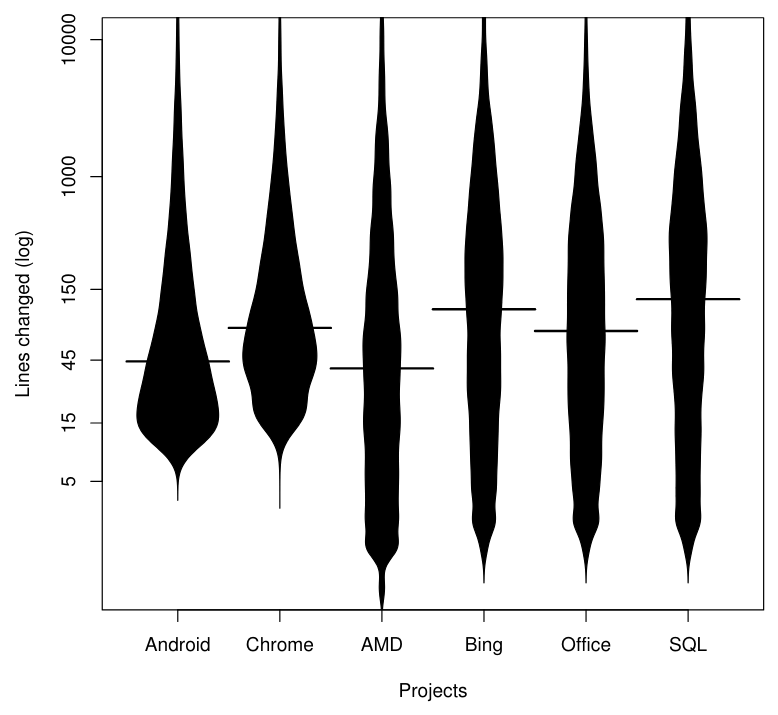
\includegraphics[width=10cm]{small_code_changes.png}
	\caption{Churn: Lines added and removed \protect\cite{rigby:review}}
	\label{fig:changes}
\end{figure}

\section{Statische Analyse}

\subsection{Grundlagen}

Die statische Analyse ist ein weiteres wichtiges Mittel zum Finden von Fehlern
und fehleranfälligen Codeabschnitten. Sie ist auch ein wichtiges Mittel zur
Qualitätsmessung.

Grundsätzlich kann jedes Dokument, welches einen rein formellen Aufbau hat,
einer statischen Analyse unterzogen werden. In der Praxis ist in fast allen
Programmierprojekten der Code selbst das einzige Dokument, was dieser
Anforderung standhält.

Die statische Analyse kann nicht alle Fehler aufdecken, da das Analysewerkzeug
nicht erkennen kann, was genau das gewünschte Verhalten genau ist. Potentielle
Fehler können aufgedeckt werden, da diese oftmals denselben Mustern folgen. Die
statische Analyse kann jedoch als einziger automatisierbarer Test Fehler wie
das Nichteinhalten von gesetzten Standards, Konventionen und Richtlinien
entdecken.

\subsection{Werkzeuge}

Falls eine kompilierte Programmiersprache genutzt wird, wird durch den Compiler
selbst Syntaxverstöße und unerlaubte Operationen bei Kompilierzeit abgefangen.
Dies stellt auch eine Form der statischen Analyse dar. Ansonsten überprüfen
Werkzeuge wie z.B. clang-tidy \cite{clang:tidy} den Einhalt von sonstigen
Konventionen oder Standards. Die einzelnen Werkzeuge sind in der Regel
sprachspezifisch. Diese müssen oft im Vorhinein mit den gewünschten
Sprachkonventionen konfiguriert werden.

Einige Beispiele für mögliche Anwendungsfälle:
\begin{enumerate}
	\item Das Überprüfen von Variablen- und Funktionsnamen.
	\item Das Finden von ungenutzten Parametern und Variablen.
	\item Das Begrenzen der Länge von Funktionen und Dateien,oder der Länge einzelner
	      Zeilen.
	\item Das Detektieren von Totem Code, z.B. Zeilen direkt nach einem "return".
	\item Das Finden von (potentiellen) Speicherlecks, oder sonstigen Ressourcenlecks.
\end{enumerate}

\subsection{Daten- und Kontrollflussanalyse}

Die Daten- und Kontrollflussanalyse wurde sowohl von meinem Mitarbeiter Moritz
Möller genauer beschrieben, und im Detail von einer anderen Gruppe geschrieben.
Ich führe deshalb nur ein Beispiel an, wie das ganze in einem konkreten
Codebeispiel aussehen könnte. In Abbildung \ref{fig:datenfluss} ist ein
Codebeispiel dargestellt, welches folgende Fehler beinhaltet, die durch eine
Daten- und Kontrollflussanalyse identifiziert werden können:

\begin{itemize}
	\item Lesen einer Variable, bevor sie definiert wird (Z. 2 \& 3)
	\item Schreiben einer Variable, ohne, dass sie danach nochmal verwendet wird (Z. 4)
	\item Toter Code (Z. 8 ist nicht erreichbar)
\end{itemize}

\begin{figure}
	\centering
	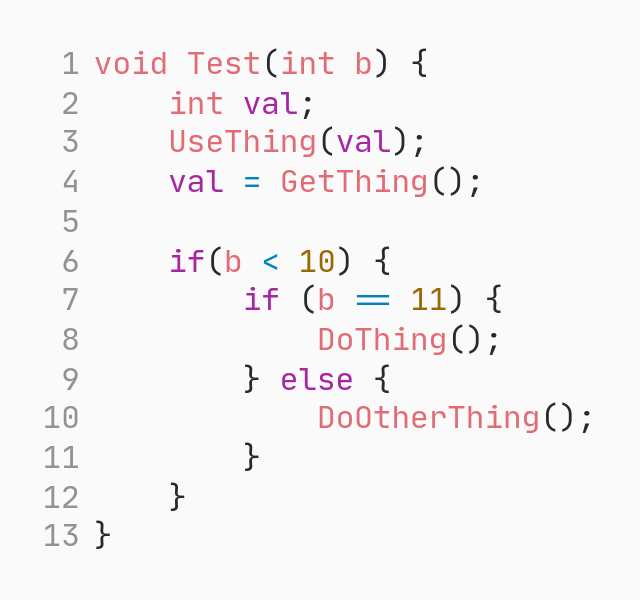
\includegraphics[width=10cm]{code_example.png}
	\caption{Codebeispiel für die Daten- und Kontrollflussanalyse} \label{fig:datenfluss}
\end{figure}

\chapter{Dynamische Tests -- Moritz Möller} \label{chap: dynamic}
In diesem Abschnitt werden die dynamischen Testmethoden untersucht. Dabei wird
auf die unterschiedlichen Kategorien eingegangen, in die diese Tests
eingeordnet werden können und ihre Anwendung anhand von Beispielen erläutert.

\section{Allgemeines}

\subsection{Definition}
Dynamische Tests werden während der Laufzeit eines Programms durchgeführt, um
dessen Funktionalitäten und Verhalten unter realen Bedingungen zu evaluieren
\cite{liggesmeyer:qualitaet}. Diese Tests können jedoch keine vollständige
Fehlerfreiheit garantieren. Eine vollständige Fehlerfreiheit könnte nur durch
einen erschöpfenden Test erreicht werden, bei dem alle möglichen Eingabewerte
getestet werden \cite{liggesmeyer:qualitaet}. Dies ist jedoch ineffizient und
bereits bei kleinen Programmen mit erheblichem Aufwand verbunden. Ein einfaches
Beispiel verdeutlicht dies: Ein 4-Byte-Integer kann über vier Milliarden
mögliche Werte annehmen, welche alle als Eingabe getestet werden müssten.

\subsection{Kategorisierung}
Eine weit verbreitete Einteilung dynamischer Testtechniken ist die Unterteilung
in White- und Black-Box Tests. White-Box-Test sind solche, die die interne
Struktur der Software untersuchen. Dabei werden insbesondere die Codestruktur
und die logische Funktionsweise getestet. \cite{hanser:qualität} Im Gegensatz
dazu bleiben bei Black-Box-Tests die internen Strukturen der Software
verborgen, was dem Namen "Black Box" entspricht. Der Code ist nicht einsehbar,
und es stehen lediglich Informationen über die Eingaben und Ausgaben des
Programms zur Verfügung. Basierend auf diesen Informationen werden Testfälle
entwickelt. Black-Box-Tests eignen sich daher besonders gut zur Überprüfung der
Spezifikationen der Software. \cite{hanser:qualität}

Diese Einteilung ist jedoch laut Peter Liggesmeyer \cite{liggesmeyer:qualitaet}
nicht ausreichend, da hierbei teilweise sehr unterschiedliche Tests in dieselbe
Kategorie eingeordnet werden. Liggesmeyer schlägt eine genauere Einteilung
anhand der Referenzen der Tests vor.

\subsection{Kategorisierung an Testreferenzen}
Die Einteilung anhand der Referenzen umfasst die folgenden Kategorien:
\begin{itemize}
	\item funktionsorientierte Testmethoden
	\item strukturorientierte Testmethoden
	\item diversifizierende Testmethoden
	\item Bereichtests
\end{itemize}
Strukturorientierte Tests werden dabei noch weiter in kontrollflussorientierte und datenflussorientierte Testmethoden unterteilt.

\section{Testmethoden}

\subsection{Funktionsorientierte Testmethoden}
Bei funktionsorientierten Tests wird anhand der vorgegebenen Spezifikationen
getestet. Der Fokus liegt darauf, sicherzustellen, dass alle spezifizierten
Funktionen wie vorgesehen arbeiten und die gewünschten Ergebnisse liefern. Da
hierbei der konkrete Code nicht betrachtet wird, können funktionsorientierte
Tests auch als Black-Box-Tests eingeordnet werden. Mit funktionsorientierten
Tests kann das Erfüllen der Spezifikationen gewährleistet werden, es ist jedoch
wahrscheinlich, dass noch nicht getesteter Code existiert. Solche Tests allein
können daher keine einwandfreie Software garantieren. Es ist zudem wichtig zu
betonen, dass die verschiedenen Testtechniken für den jeweiligen Anwendungsfall
ausgewählt werden müssen und es keine universell passenden Vorgaben für Tests
gibt. \cite{liggesmeyer:qualitaet}

\subsubsection{Zustandsorientierte Tests}
Ein Beispiel für funktionsorientierte Tests sind die zustandsorientierten
Tests. Diese prüfen das Verhalten des Programms in verschiedenen Zuständen und
bei Zustandsübergängen. Ziel ist es, sicherzustellen, dass die Software in
jedem Zustand den Spezifikationen entsprechend reagiert. Zur grafischen
Darstellung des Verhaltens werden Zustandsdiagramme erstellt (siehe Abb. 2.1).
Anschließend werden Testfälle entwickelt, die jeden Zustand und jeden
Zustandsübergang mindestens einmal überprüfen, wodurch die Testvollständigkeit
erreicht wird. \cite{liggesmeyer:qualitaet} Diese Methode ist besonders wichtig
für Systeme wie Automaten, Protokolle oder ähnliche Anwendungen.

\begin{figure}
	\centering
	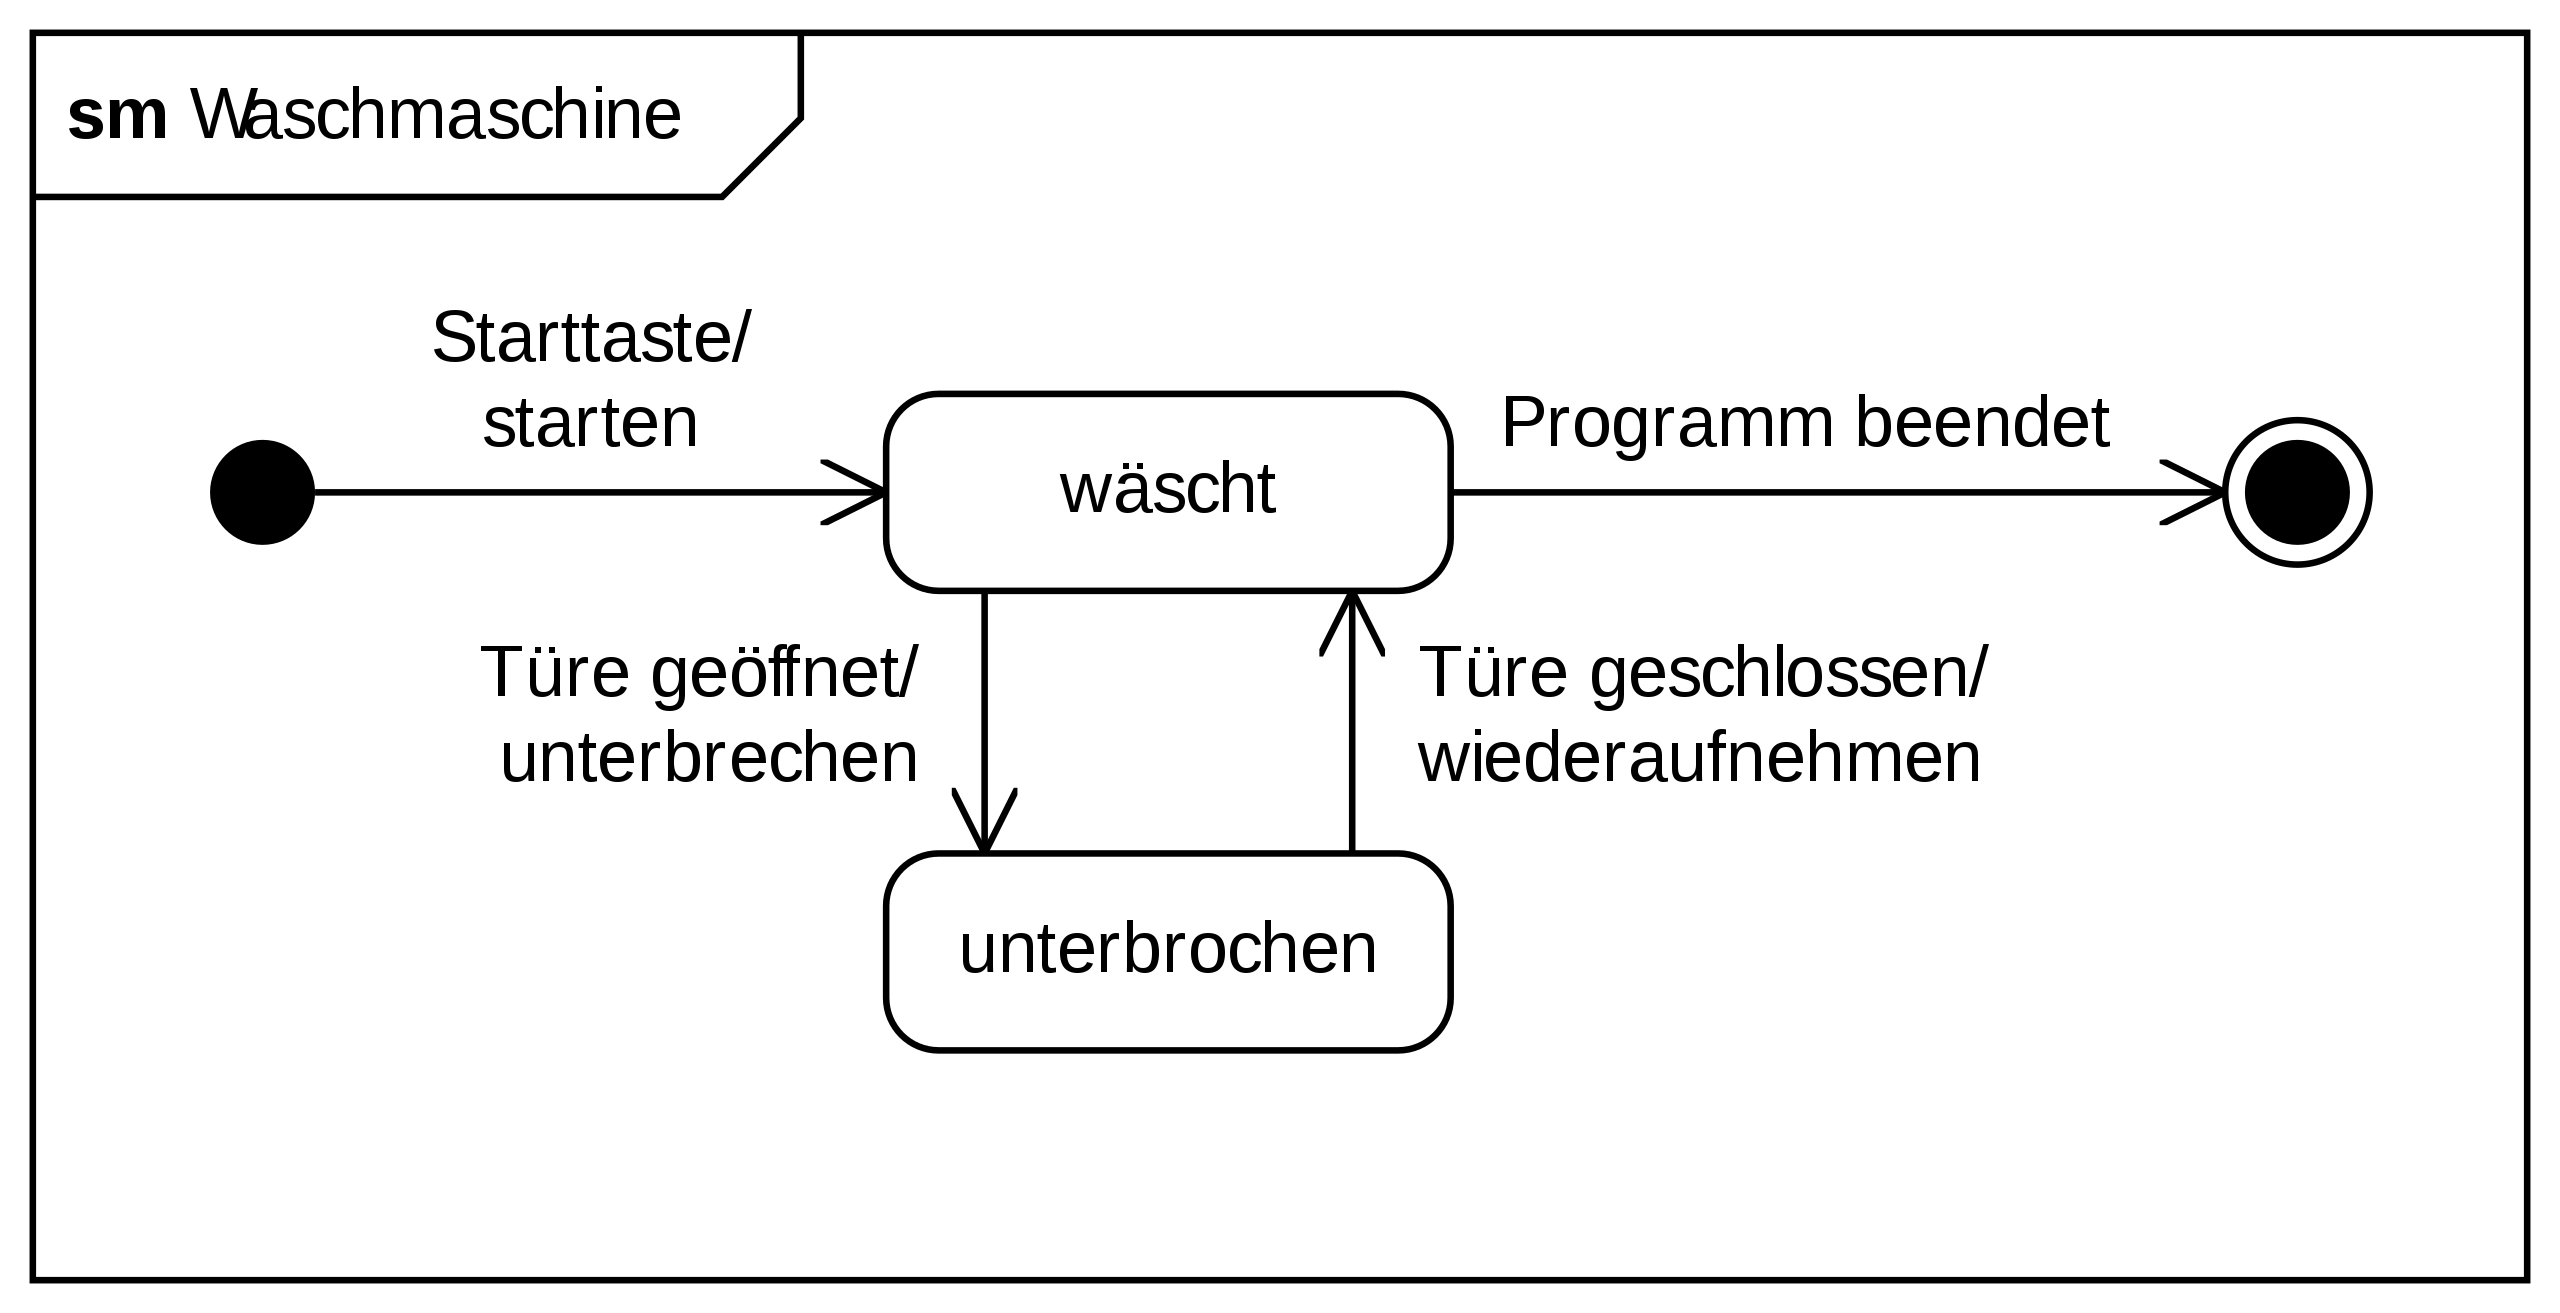
\includegraphics[width=10cm]{UML-Zustandsdiagram.png}
	\caption{Beispiel für ein UML-Zustandsdiagramm \cite{wikipedia:Zustandsdiagramm}}
\end{figure}

\subsection{Strukturorientierte Testmethoden}

Strukturorientierte Testmethoden sind im Gegensatz zu den funktionsorientierten
Methoden darauf ausgelegt, die interne Struktur des Codes zu testen
\cite{liggesmeyer:qualitaet}. Somit können sie als Teilmenge der
White-Box-Tests angesehen werden. Diese Testmethoden lassen sich weiter in
kontrollflussorientierte und datenflussorientierte Tests unterteilen.

\subsubsection{Kontrollflussorientierte Testmethoden}

Kontrollflussorientierte Tests sind darauf ausgelegt, Kontrollstrukturelemente
abzudecken. Dabei wird die Verarbeitungslogik, wie Anweisungen, Schleifen und
Verzweigungen, geprüft. Dies kann grafisch mithilfe eines Kontrollflussgraphen
(siehe Abb. 2.3) dargestellt werden. \cite{liggesmeyer:qualitaet}

\subsubsection{Zweigüberdeckungstest}
Ein hilfreicher kontrollflussorientierter Test ist der Zweigüberdeckungstest.
Bei diesem Test muss jede Kante in einem Kontrollflussgraphen durchlaufen
werden, um die Fehlerfreiheit der Software zu gewährleisten.
\cite{liggesmeyer:qualitaet}

\begin{figure}
	\centering
	\begin{minipage}{0.49\textwidth}
		\centering
		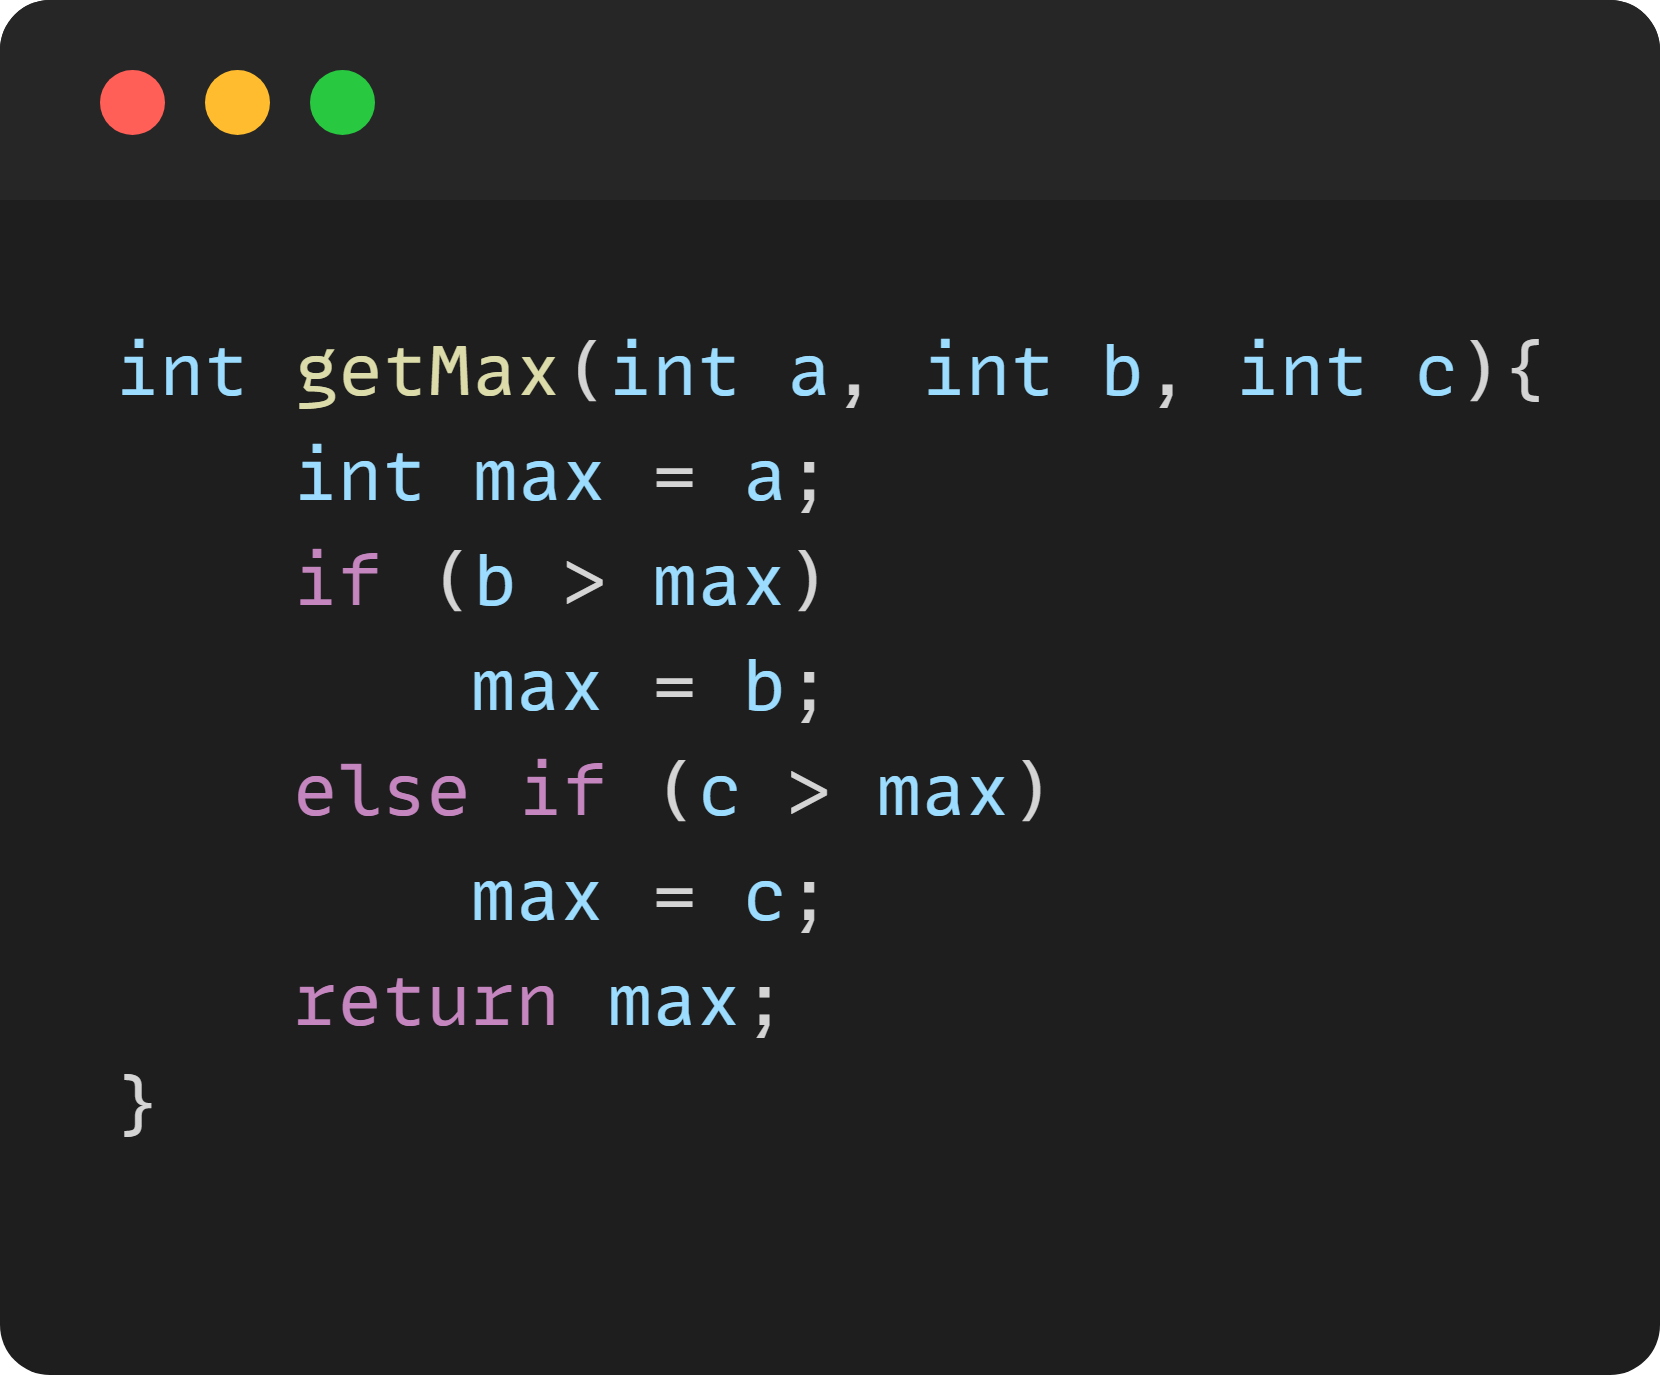
\includegraphics[width=1\textwidth]{getMax_Bsp.png}
		\caption{Ein Codebeispiel}
	\end{minipage}\hfill
	\begin{minipage}{0.49\textwidth}
		\centering
		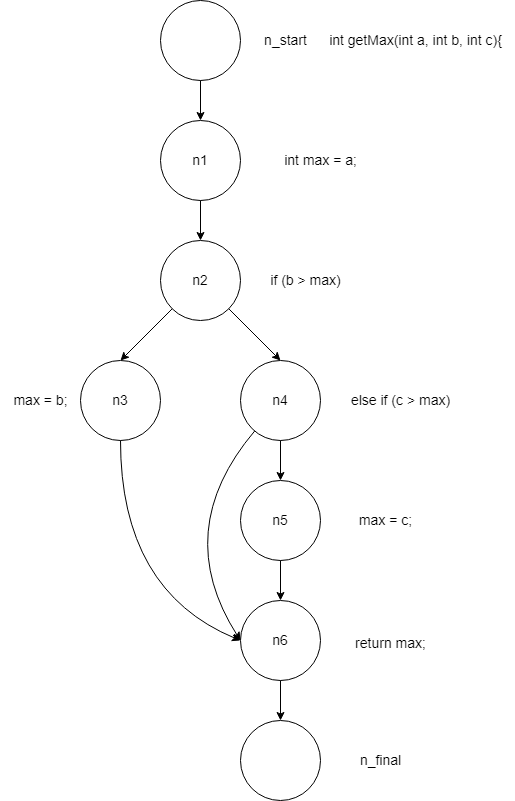
\includegraphics[width=1\textwidth]{Zweig_Dia.png}
		\caption{Der dazugehörige Kontrollflussgraph}
	\end{minipage}
\end{figure}

Konkret an einem Beispiel sieht das wie folgt aus: Für die Funktion aus Abb.
2.2 lässt sich der Kontrollflussgraph Abb. 2.3 ableiten. Mit diesem lässt sich
leicht ermitteln, dass drei Testfälle abzudecken sind:

\begin{enumerate}
	\item „b > a“ und „b >= c“ (erste if-Bedingung wahr)
	\item „c > a“ und „c > b“ (erste if-Bedingung falsch, else if wahr)
	\item „a >= b“ und „a >= c“ (erste und zweite Bedingung falsch)
\end{enumerate}

Diese Fälle können dann mit passenden Eingabewerten getestet werden. Zum
Beispiel:

\begin{enumerate}
	\item „a = 3, b = 5, c = 2“
	\item „a = 2, b = 3, c = 5“
	\item „a = 5, b = 3, c = 2“
\end{enumerate}

\subsubsection{Datenflussorientierte Testmethoden}
Datenflussorientierte Testmethoden konzentrieren sich auf die Prüfung
sämtlicher Datenzugriffe in einem Programm. Das Ziel ist dabei sicherzustellen,
dass die Nutzung und der Fluss von Variablen und Datenstrukturen im Code
korrekt und fehlerfrei sind. Dies ist besonders nützlich für objektorientierten
Code, da sich bei diesem die Programmierung um Datenobjekte orientiert und
einen zentralen Aspekt darstellen. Die Korrektheit der Ausgabewerte solcher
Tests wird anhand der Spezifikation geprüft. \cite{liggesmeyer:qualitaet}

Für datenflussorientierte Tests werden folgende Definition für
Variablenzugriffe verwendet: „Definition“ (kurz „def“) für schreibenden
Zugriff, „computational use“ (kurz „c-use“) für den lesenden Zugriff mit
Benutzung für Berechnungen oder Wertzuweisungen und „predicate use“ (kurz
„p-use“) für den lesenden Zugriff mit Benutzung für Bedingungen.
\cite{liggesmeyer:qualitaet}

Zur grafischen Darstellung wird ein erweiterter Kontrollflussgraph verwendet.
Bei diesem wurden Datenflussattribute hinzugefügt (siehe Abb. 2.5). In diesem
werden am Anfang und am Ende jeweils globale Variablen aufgeführt. Mit global
ist in diesem Fall außerhalb des betrachteten Blocks gemeint. Die „p-uses“
werden im Graphen an die abgehenden Kanten von Knoten für Bedingungen
geschrieben und „c-uses“ und „def“ an die jeweiligen Knoten.
\cite{liggesmeyer:qualitaet}

\subsubsection{Def/Uses-Test}
Der Def/Uses-Test als datenflussorientierter Test wird die Verbindung und der
Fluss von Daten überprüfen. Dies geschieht an den Stellen wo Variablen
definiert („defs“) oder verwendet werden („uses“). Der Test ermöglicht die
Identifizierung nicht referenzierter und uninitialisierter Variablen, sowie das
Erkennen von falschen oder unerwarteten Datenflüssen.
\cite{liggesmeyer:qualitaet}

\begin{figure}
	\centering
	\begin{minipage}{0.49\textwidth}
		\centering
		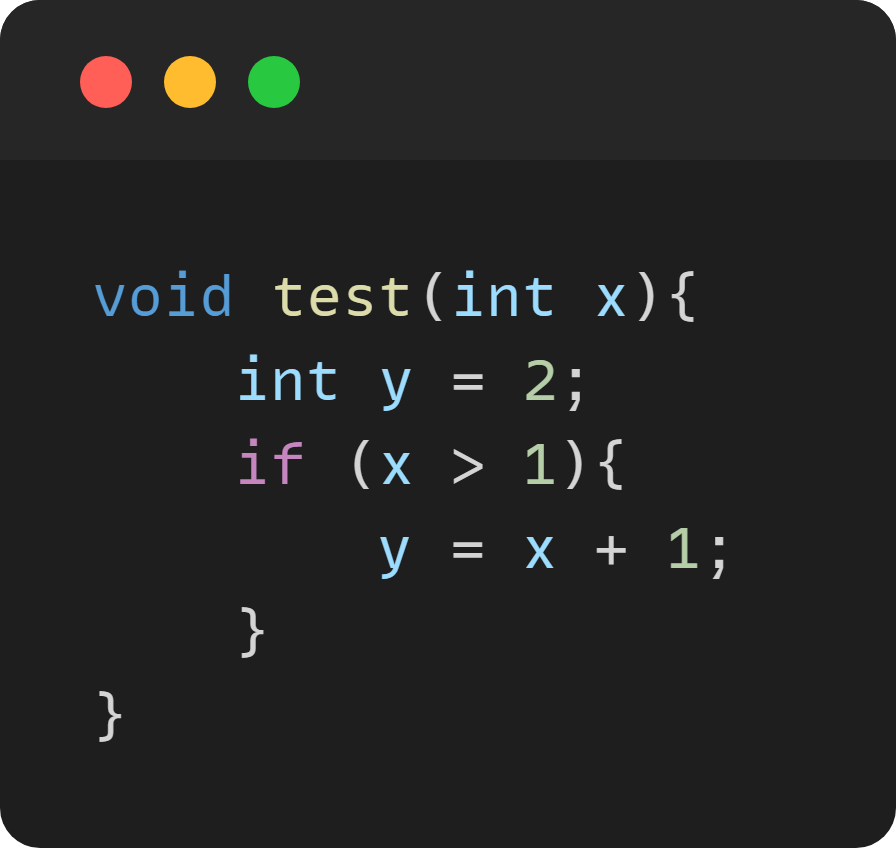
\includegraphics[width=1\textwidth]{test_Bsp.png}
		\caption{Ein Codebeispiel}
	\end{minipage}\hfill
	\begin{minipage}{0.49\textwidth}
		\centering
		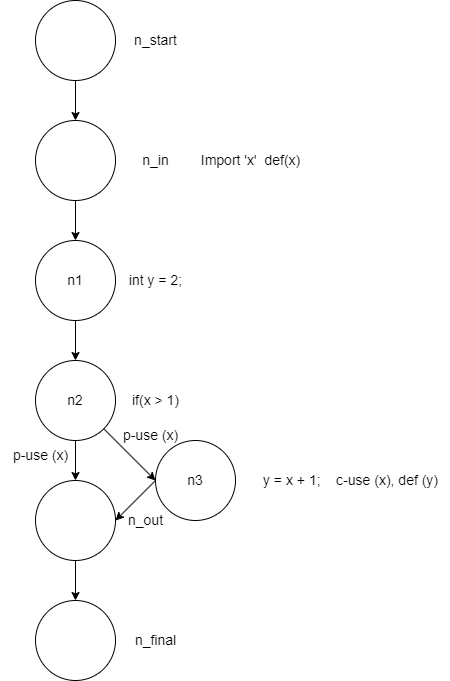
\includegraphics[width=1\textwidth]{DefsUses_Dia.png}
		\caption{Der dazugehörige erweiterte Kontrollflussgraph}
	\end{minipage}
\end{figure}

Die Durchführung des Def/Uses-Tests erfolgt anhand eines konkreten Beispiels
wie folgt: Zunächst wird der Kontrollflussgraph basierend auf dem zu testenden
Quellcode erstellt (vgl. Abb. 2.4 und 2.5). Anschließend werden die "defs" und
"uses" der Variablen im Programm identifiziert. Im vorliegenden Beispiel sind
dies die Definitionen und Verwendungen der Variablen x und y:

\begin{itemize}
	\item Variable x:
	      \begin{itemize}
		      \item Defs: Import (Zeile 0)
		      \item Uses: if (x > 1) (Zeile 2), y = x + 1 (Zeile 3)
	      \end{itemize}
	\item Variable y:
	      \begin{itemize}
		      \item Defs: int = 2; (Zeile 1), y = x + 1; (Zeile 3)
		      \item Uses: keine
	      \end{itemize}
\end{itemize}

Daraus lassen sich dann die „Definition-Use“ (DU)-Pfade festgestellt. In dem
Fall hat nur die Variable x zwei Pfade und zwar:

\begin{enumerate}
	\item Zeile 0 zu Zeile 2
	\item Zeile 0 zu Zeile 3
\end{enumerate}

Die Variable y hat keine Pfade, da diese nur definiert, aber nicht benutzt
wird. Anhand der DU-Pfade können nun Testpfade entworfen werden. Zum Beispiel:

\begin{itemize}
	\item x = 2, dann muss y am Ende der Funktion den Wert 3 haben
	\item x = 1, dann muss y den Wert 2 besitzen
\end{itemize}

\subsection{Diversifizierende Testmethoden}
Eine heute praktisch kaum noch genutzte Kategorie von Testmethoden sind die
diversifizierenden Tests. Hierbei werden unterschiedliche Versionen einer
Software gegeneinander getestet. Dieser Ansatz vereinfacht die Bewertung der
Korrektheit gegenüber den Spezifikationen, da die unterschiedlichen
Abstraktionsebenen der Implementierungen wegfallen
\cite{liggesmeyer:qualitaet}. In der modernen Softwareentwicklung wird der
Aufwand beziehungsweise die Kosten für solche Tests jedoch als zu hoch
eingeschätzt, weshalb sie meist vermieden und durch andere Testmethoden ersetzt
werden.

\subsubsection{Back to Back Test}
Ein prominentes Beispiel für einen diversifizierenden Test ist der
Back-to-Back-Test. Bei diesem Verfahren werden mehrere Programmversionen aus
derselben Spezifikation von unterschiedlichen Entwicklern erstellt. Diese
Versionen werden anschließend gegeneinander getestet, um potenzielle Fehler
aufzudecken. Hierbei können jeweils dieselben Testdatensätze verwendet werden.
\cite{liggesmeyer:qualitaet}

\subsection{Bereichstests:}
Die Bereichstests stellen eine Kombination einfacher fehlerorientierter
Testtechniken dar. \cite{liggesmeyer:qualitaet}

\newpage

\subsubsection{Pfadbereichstest}
Ein Beispiel für einen Bereichstest ist der Pfadbereichstest. Dieser zielt
darauf ab, Bereichsfehler aufzudecken. Unter Bereichsfehlern versteht man
hierbei die fehlerhafte Definition von Eingabebereichen, z.B. bei
if-Bedingungen, die zur Ausführung falscher Programmpfade führen kann. Da
Fehler oft an den Bereichsgrenzen auftreten, werden diese besonders getestet.
\cite{liggesmeyer:qualitaet}

Der Pfadbereichstest kombiniert den strukturorientierten Pfadüberdeckungstest
mit der fehlerorientierten Grenzwertanalyse und der strukturorientierten
Äquivalenzklassenbildung. \cite{liggesmeyer:qualitaet}

Die Durchführung erfolgt wie folgt: Zunächst werden Eingabewerte zum Erreichen
eines bestimmten Pfades getestet. Dies ermöglicht die Festlegung der Bereiche,
die zu diesem Pfad führen sollen (sog. Pfadbedingung). Wenn keine Eingabewerte
für einen Pfad gefunden werden können, ist dieser nicht ausführbar und es liegt
ein Fehler in der Programmierung vor. \cite{liggesmeyer:qualitaet}

\chapter{Fazit}

Statische und dynamische Testmethoden haben grundsätzlich unterschiedliche
Anwendungsbereiche, aber ergänzen sich sehr gut. Statische Tests fokussieren
sich primär auf Codequalität, während dynamische Tests sich primär auf
Codekorrektheit beschränken. Beide Überkategorien an Tests sind auf jeden Fall
unabdingbar für den langfristigen Erfolg eines Programmierprojekts.

\printbibliography

\end{document}
